\chapter{Alarm}
\section{Inleiding}
In de alarm module wordt een led aangestuurd, die 15 minuten voor de ingestelde tijd in de main controller begint met branden en steeds feller wordt naarmate de tijd verstrijkt. Als de huidige tijd gelijk is aan de ingestelde tijd brandt de led op z'n felst en gaat er een geluid af, totdat er een knop wordt ingedrukt.

\section{Specificaties}
\subsection{Ingangen}
\begin{itemize}[nolistsep]
\item Klok, standaard input.
\item Reset, standaard input.
\item Tijd-uur, huidige tijd in uren.
\item Tijd-minuut, huidige tijd in minuten.
\item Wekker-uur, uur ingesteld in de main controller.
\item Wekker-min, minuten ingestels in de main controller.
\item Sec, seconde signaal gegenereerd in de DCF controller.
\item Knop, alarm uitschakelen.
\end{itemize}

\subsection{Uitgangen}
\begin{itemize}[nolistsep]
\item PWM-signaal, signaal om de led aan te sturen.
\item Geluid, signaal om een geluid af te laten gaan.
\end{itemize}

\subsection{Gedrag}
Het alarm moet een bepaalde tijd voordat de wekker is ingesteld aangaan, nu gekozen voor 15 minuten.
Er wordt 15 minuten van de ingestelde tijd afgetrokken. Zodra die tijd gelijk is aan de huidige tijd komt er een signaal (licht) aan bij het gedeelte wat voor een pwm signaal zorgt.
In dat gedeelte wordt een pwm signaal gegenereerd dat elke 15 seconde breder wordt. Dit wordt gedaan door in een counter 15 seconde te tellen. Elke 15 seconde wordt de variable "lenght" kleiner. Deze begon op 64 en wordt vergeleken met een andere counter die elke klokflank telt, tot 64. Als de counter groter of gelijk is aan "length" dan is het pwm-signaal hoog. 
Als 15 minuten zijn verstreken na het aangaan van de led, dus de ingestelde tijd is gelijk aan de huidige tijd, brandt de led op z'n felst. Ook zal dan een "geluid" signaal naar '1' gaan. Dit blijft zo totdat de knop wordt ingedrukt of alles wordt gereset.

\subsection{FSM}
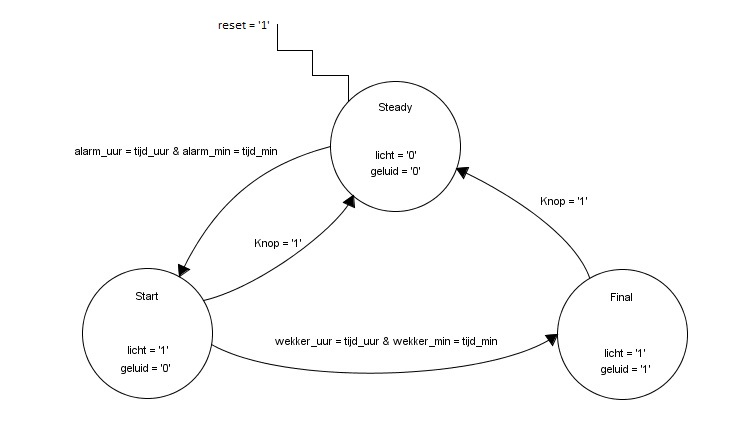
\includegraphics[width=\textwidth,height=\textheight,keepaspectratio]{FSM/alarm-compare-fsm.jpg}